\documentclass[11pt,a4paper,english]{article}

\usepackage{default_packages}
\usepackage{pdfpages}
\usepackage{prog2tex}

%\pagestyle{fancy}
\cfoot{}
\rfoot{Page \thepage\ of \pageref{LastPage}}
 
\begin{document}
	\begin{titlepage}
		{\centering \parindent=0pt
		\newcommand{\HRule}{\rule{\textwidth}{1mm}}
		\vspace*{\stretch{1}} \LARGE%\bfseries
		Real time rendering of skeletal implicit surfaces.\\[0.7cm]
		\large 
		
			Olivier Rouiller\\
			\normalsize 
			IMM-M.Sc.-2011-70
			 
   		
   		}

		\vspace*{\stretch{2}} \normalsize %
   		\begin{wrapfigure}{r}{0.1\textwidth}
   			\vspace{-35pt}
   			\begin{center}
   				
\includegraphics[scale=0.3]{../../figs/DTU.pdf}
   			\end{center}
   		\end{wrapfigure}
		
		\noindent Technical University of Denmark\\
					Informatics and Mathematical Modelling\\
					Building 321, DK-2800 Kongens Lyngby, Denmark\\
					Phone +45 45253351, Fax +45 45882673\\
					reception@imm.dtu.dk\\
					www.imm.dtu.dk\\
   		\FloatBarrier
\end{titlepage}
\newpage


	\section{Preface}

This report summarizes and presents my work during my master project at the Computer graphics and Image analysis at the Technical University of Denmark. This six-month work was focused on geometric modelling and rendering with implicit surfaces. My objective was to study recent methods for ray-tracing implicit surfaces on the GPU and to adapt them to render models modelled by their skeleton.
The motivation was to use the simplicity that provide skeletal implicit surfaces to model surfaces without having to tessellate them as it is usually done. In order to be interesting, the method had to allow animation and texturing, thus being usable to render characters for example.

The first part of this report presents the most relevant results of my work, it is presented on the form of a conference article. I review here the bibliography that is relevant to this problem. I present the surface representation that I choose to create the models and the algorithm that I used to render the surfaces. I also present a method to animate the models using a hierarchical bone data structure and a method to allow texturing of the models with user control.

In Appendix A, I present some work that I did on using a bounding volume hierarchy to accelerate the ray-tracing algorithm. This work did not provide a real advantage on the efficiency of the algorithm for the size of the models that I used. Hierarchical data structures are indeed not convenient to use on the GPU and traversing the BVH induces an overhead in branching and additional computation to test the ray against the bounding boxes of the node. However, as it is presented in the article, the algorithm suffers from a poor scalability and using a BVH could become an advantage for complex models or for a scene with several models. Therefore I provide in appendix a description of the algorithm and some implementation details.

\newpage
\section{Acknowledgements}


I would like to thank my supervisor on this project Jakob Andreas B{\ae}rentzen for the original idea proposal, for the advises along the project and for the quality of his teachings. I would like to thank my family and friends for their support. I would like to thank the IMM staff and the staff from the Computer Graphics and Image Analysis department for making IMM an attractive environment to study.

\newpage
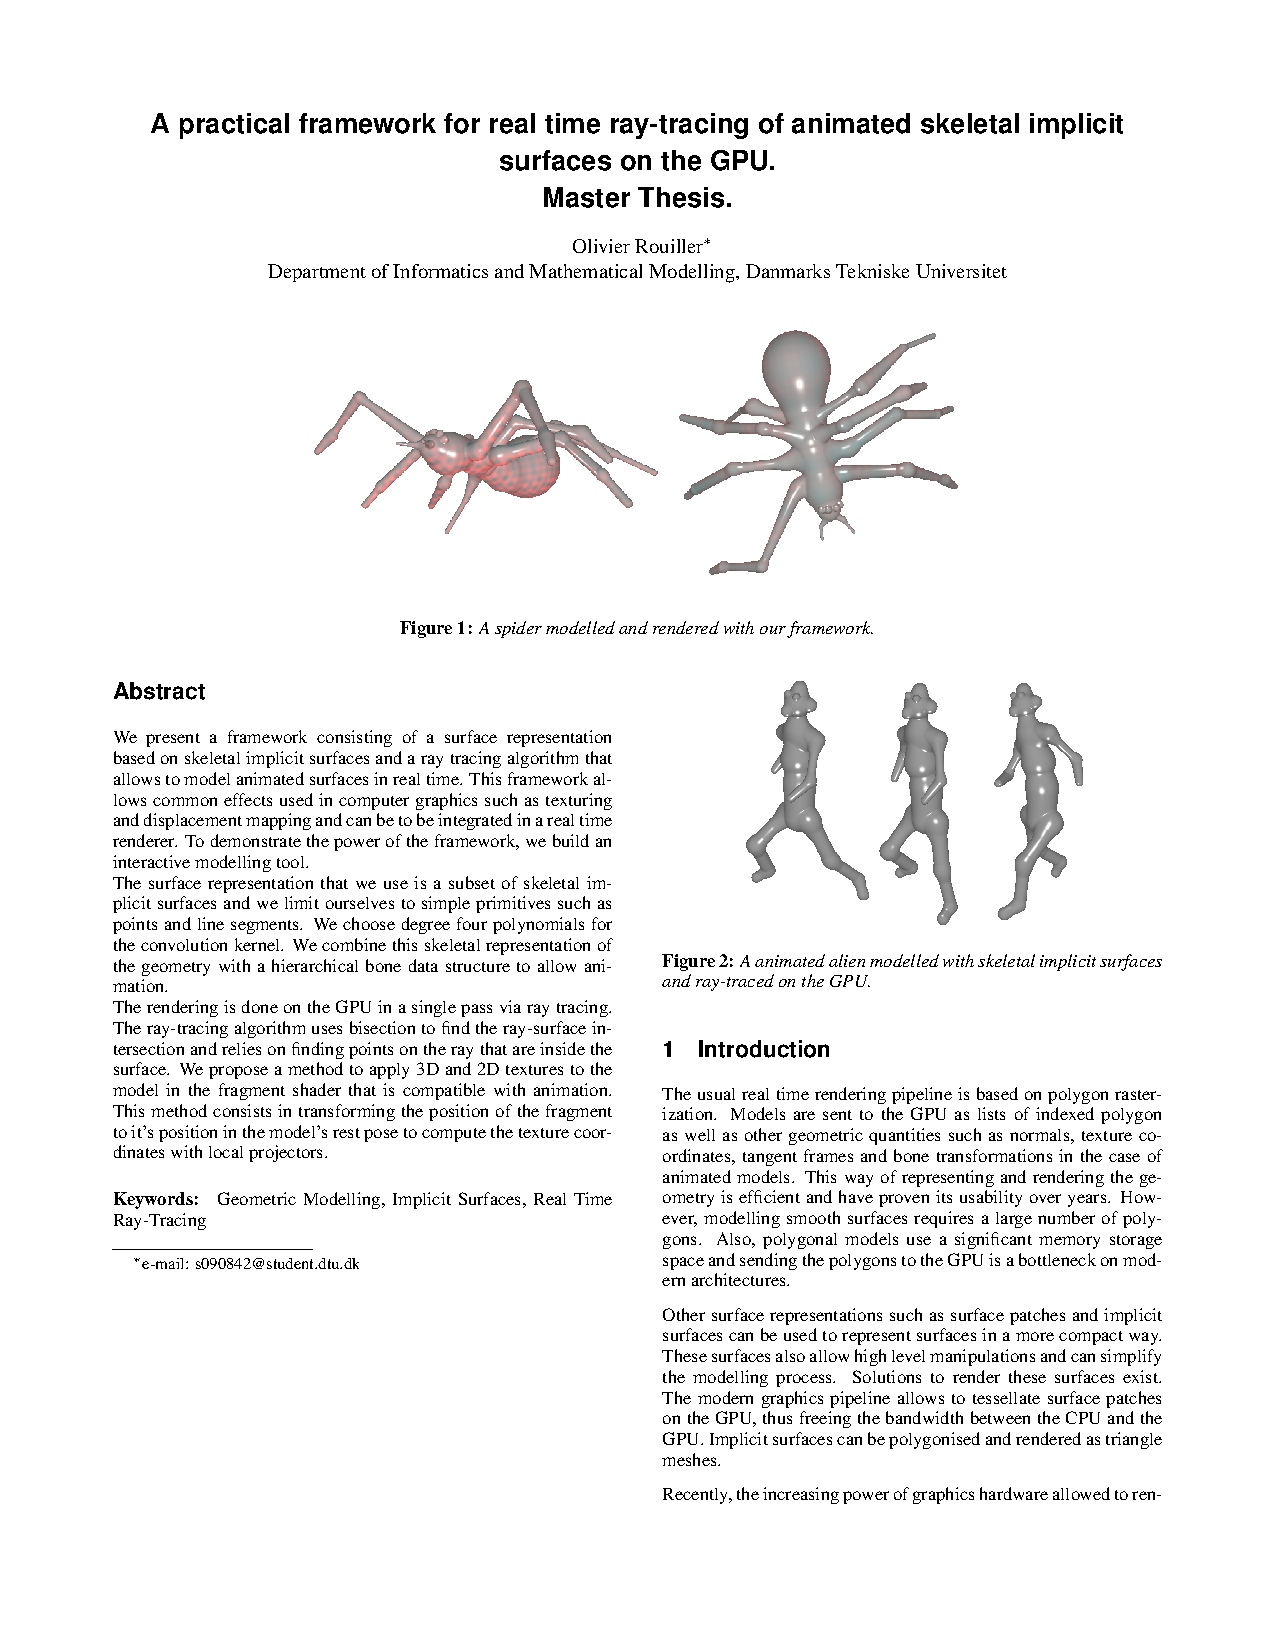
\includepdf[pages=1-8]{../Paper/template.pdf}
\appendix
\section{Towards a better scalability of the ray-tracing algorithm.}

The algorithm to find the ray surface intersections that we presented is relatively fast but suffers from a poor scalability.
The first reason is that when discarding the non contributing primitives, we evaluate the entire function for each test.
Also, when we search for intersection by bisection, we evaluate the potential of all the primitives that whose surface of influence intersect the ray. To address this issue, \cite{Gourmel-2010-FBVH} use a fitted BVH. Using a bounding volume hierarchy allows to reduce the number of primitives tested when we compute the first interval for the bisection.

I tried to adapt this algorithm for my surface representation but I was not able to achieve better performances with it. However, this technique, carefully implemented and optimised could allow to increase the scalability of the algorithm. 

\subsection{Building the BVH}

\subsubsection{Overview of the algorithm.}

The BVH that we build is a BVH where the leaf nodes contain references to the primitives that have an influence inside their axis aligned bounding box. The BVH is built from top to bottom and at each stage, we split the AABB of the node and distribute to the two children the primitives of the node. Finding the splitting plane should be done using a Surface Area Heuristic (SAH).
The algorithm evaluates the cost of traversing the BVH during ray-tracing of several possible splits and choose the one that has the least heuristic cost.

When splitting the node, primitives are distributed to the left child or to the right child according to their position with respect to the splitting plane. Then the primitives of the right child are tested for intersection with the primitives of the left child. The primitives that do intersect are added to the right child as split primitives. 

Finally, the AABBs of the children are computed as the AABB of all the primitives that they contain intersected with the half AABB of the parent node.
This way, the nodes do not overlap, are tightly enclosing the primitives that have an influence inside and contains references to these primitives.

This property is convenient to be used with our bisection scheme.


\subsubsection{Memory layout}

The BVH has to be transferred to the GPU for ray traversal. As suggested in \cite{}, we transfer it as texture memory.
To fit the memory layout of the texture memory, the BVH is encoded in a plain array where the children of a node $i$ are located at indices $2i+1$ and $2i+2$.

We choose to encode the BVH in a 4 component floating point texture. We store a node in two pixels, one for each corner of the AABB.
The w component of the pixels are used to store a flag, it's value is -1 if the node is not a leaf, otherwise, it is a index to the list of the primitives contained in the node.

We also write in the texture after the tree the lists of primitives, we allocated two pixels to store the indices to the metaballs and two pixels to store the indices to the metatubes. This way a node can contain at most 8 metaballs and 8 metatubes. 

\subsection{Traversing the BVH}

The BVH is traversed from front to back, when we reach a leaf node, we try to find a point on the ray and inside the surface as described in the article. I no such point is found, we backtrack and visit other node farther on the ray. This algorithm requires to maintain a stack where we push the indices of the nodes that should be visited. Listing \ref{travers} shoxs the code used to traverse the BVH on the GPU. It returns the node where the ray intersects the surface if any. It also loads in global variables the primitives that have an influence inside the node and caches the point inside the surface used to initialize the bisection.

\bibliography{../references} 
\bibliographystyle{plain}

\begin{algorithm}                      % enter the algorithm environment
\caption{Traversing the BVH}          % give the algorithm a caption
\label{travers}                           % and a label for \ref{} commands later in the document
\begin{minipage}{0.9\textwidth}%
\tiny
\CPP
int RayIntestectsBVH(vec3 origine, vec3 dir){
	vec4 bottomC, topC;
	top = 0;
	int node = 0, c1 =0, c2 = 0;
	
	//push the BVH top node on the stack	
	push(node);
	while(top > 0){
		//First non expanded node
		node = pop();
		
		//Load the AABB of the node
		bottomC = nodeBottom(node);
		topC = nodeTop(node);
		
		//If this is a leaf check for intersection with the surface
		if(bottomC.w != -1.0 || topC.w != -1.0){
			//This test loads the primitives if the node and tries to find a point inside the surface.
			//The test is positive if such a point is found.
			if(rayIntersectsSurfaceInNode(origine, dir, node)) return node;
		}else{
			//Otherwise expand
			c1 = child1(node);
			c2 = child2(node);
			//Distances from the eye to the AABBS intersection
			float d1;
			float d2;
			
			//Test c1 for intersection
			bottomC = nodeBottom(c1);
			topC = nodeTop(c1);
			bool c1Intersects = RayIntestectsAABB(origine, dir, bottomC.xyz, topC.xyz, d1);
			//Test c2
			bottomC = nodeBottom(c2);
			topC = nodeTop(c2);
			bool c2Intersects = RayIntestectsAABB(origine, dir, bottomC.xyz, topC.xyz, d2);
			
			//Push the children if their intersect by order of distance to the eye
			if( c1Intersects ){
				if( c2Intersects ){
					if( d1 <= d2 ){
						push(c2);
						push(c1);
					}else{
						push(c1);
						push(c2);
					}
				}else
					push(c1);
			}else if( c2Intersects )
				push(c2);
		}
	}
	return -1;
}
\END\PROGb{}

\end{minipage}%
\end{algorithm}

\end{document}
